\section{Methods}\label{sec:methods}

% =========================================================================
%
% EB writes here - this is method but parts of it can also be included in introduction.

\subsection{Vision Transformers} \label{ssec:vit}
In 2017, a novel architechture for deep learning was introduced with the infamous article 
"Attention is all you need" \cite{attention}. This architechture is today known as the 
tranformer, which laid the basis for the curren AI wave which includes major 
names such as ChatGPT, Dal-E and AlphaFold 2.

The transformer architechture was originally thought to replace recurrent neural networks (RNN)
as the model of choice for translation of text. The model had several novel ways to train a network,
but the main focus was on the attention mechanism. We will not go into detail on the attention
mechanism here, but it is worth a mention that this concept introduced in 2014 \cite{first_attention}
provides the network with more context for each data point that it tries to predict, which is one
of the aspects that made transformers superior in predicting and later producing full sentences. 

Only three years after the first transformer architechture was introduces, the article 
"An Image is Worth 16x16 Words: Transformers for Image Recognition at Scale" \cite{first_vit}
introduced the first functional transformer trained on images, and it was baptized as a Vision
Transformer (or ViT for short). The authors demonstrate how a ViT outperforms classical 
deep learning methods such as convultional neural networks (CNN), not only in scores but also
in computational training costs.

A ViT splits an image into even sized, non-overlapping patches, which are then linearily embedded
as token representations. These tokens are then fed into the regular transformer architechture with 
their positional embeddings. The previously mentioned attention mechanism is then used during training
so that the model consideres spatial relationships within and between patches. The authors of this 
report will not pretend to understand the ViT completely, but we provide the reader with all sources
to fully comprehend this novel architechture, and present the original layout of a ViT in Figure \ref{fig:ViT}

\begin{figure}[H]
    \centering
    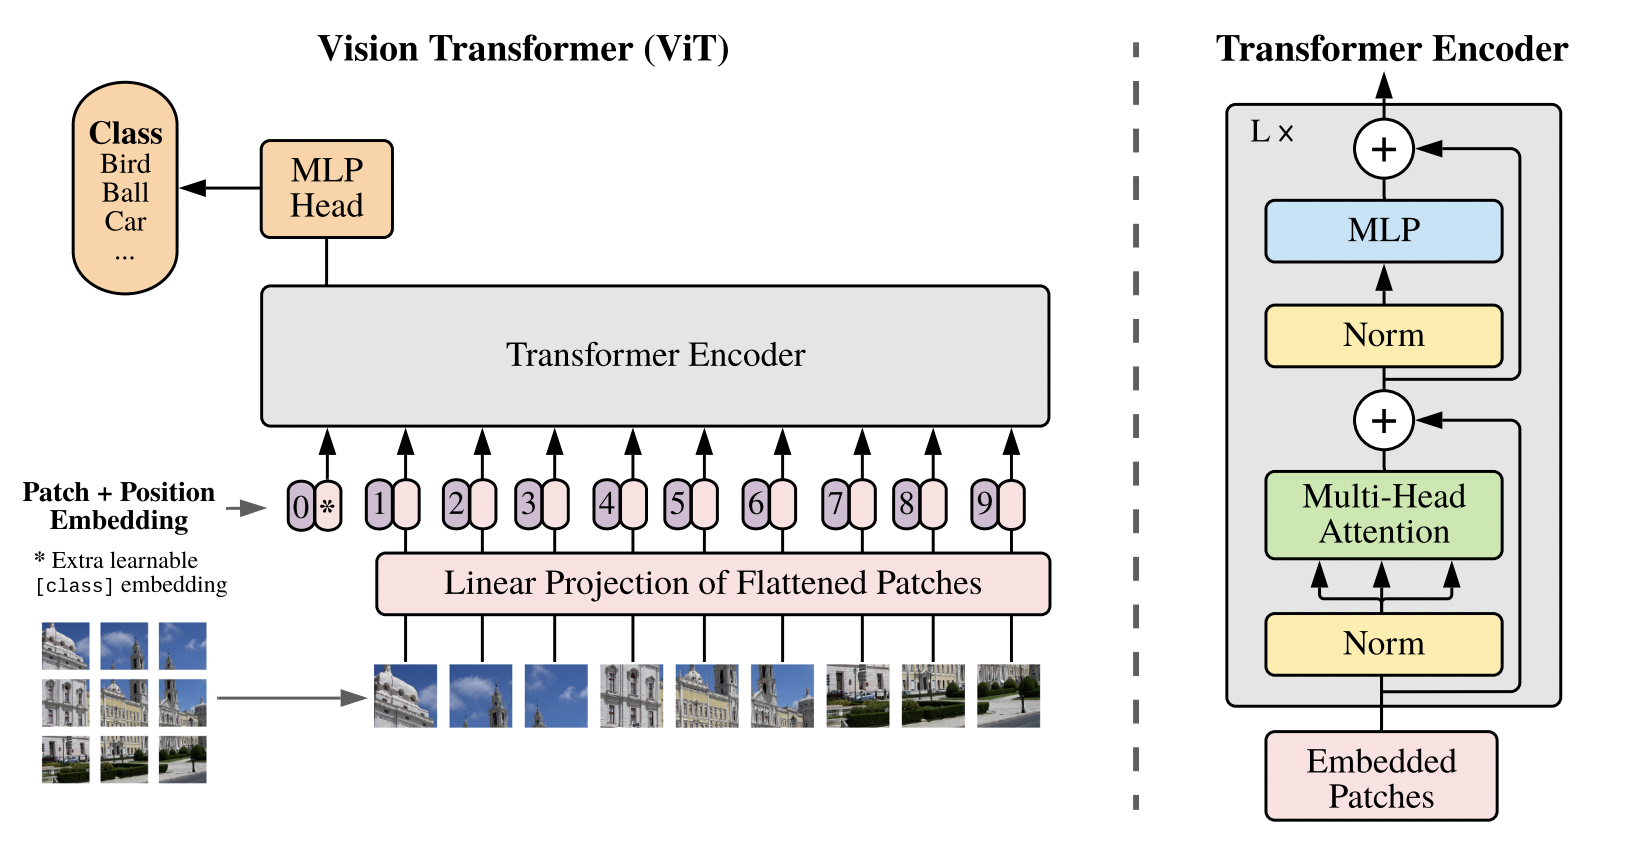
\includegraphics[width=1.1\linewidth]{examples/tests_eb/figs//Users/ellen-beatetysvaer/Documents/H24/FYS-STK/ml_github/FYS-STK4155-Project3/examples/tests_eb/figs/Skjermbilde 2024-11-26 kl. 15.15.54.png}
    \caption{Vision Transformer layout as presented from it's original paper \cite{first_vit}}
    \label{fig:ViT}
\end{figure}




%
% =========================================================================

% =========================================================================
%
% Janita writes here
%
% =========================================================================

% =========================================================================
%
% Even writes here
%
% =========================================================================